\section{\mi との連携}
\label{sec:misskey1}
    \subsection{\mi 側の設定}
    \label{sec:misskey2}
        \subsubsection{\accessToken の発行}
        \label{sec:misskey3}
            \begin{enumerate}
                \item \nowplaying したい\mi サーバーで二要素認証の設定が必要な場合は、\href{https://support.misskey.io/hc/ja/articles/9354169842191-%E4%BA%8C%E8%A6%81%E7%B4%A0%E8%AA%8D%E8%A8%BC%E3%81%AE%E8%A8%AD%E5%AE%9A%E3%81%AB%E3%81%A4%E3%81%84%E3%81%A6}{こちら}を参考にあらかじめ設定を行ってください。
                \label{item:misskey1}
                \item 設定画面の\ttbox{Misskey接続設定}を押下して、設定項目を展開してください。
                \label{item:misskey2}
                    \begin{figure}[htbp]
                        \begin{minipage}[b]{0.45\linewidth}
                            \centering
                            \fbox{
                                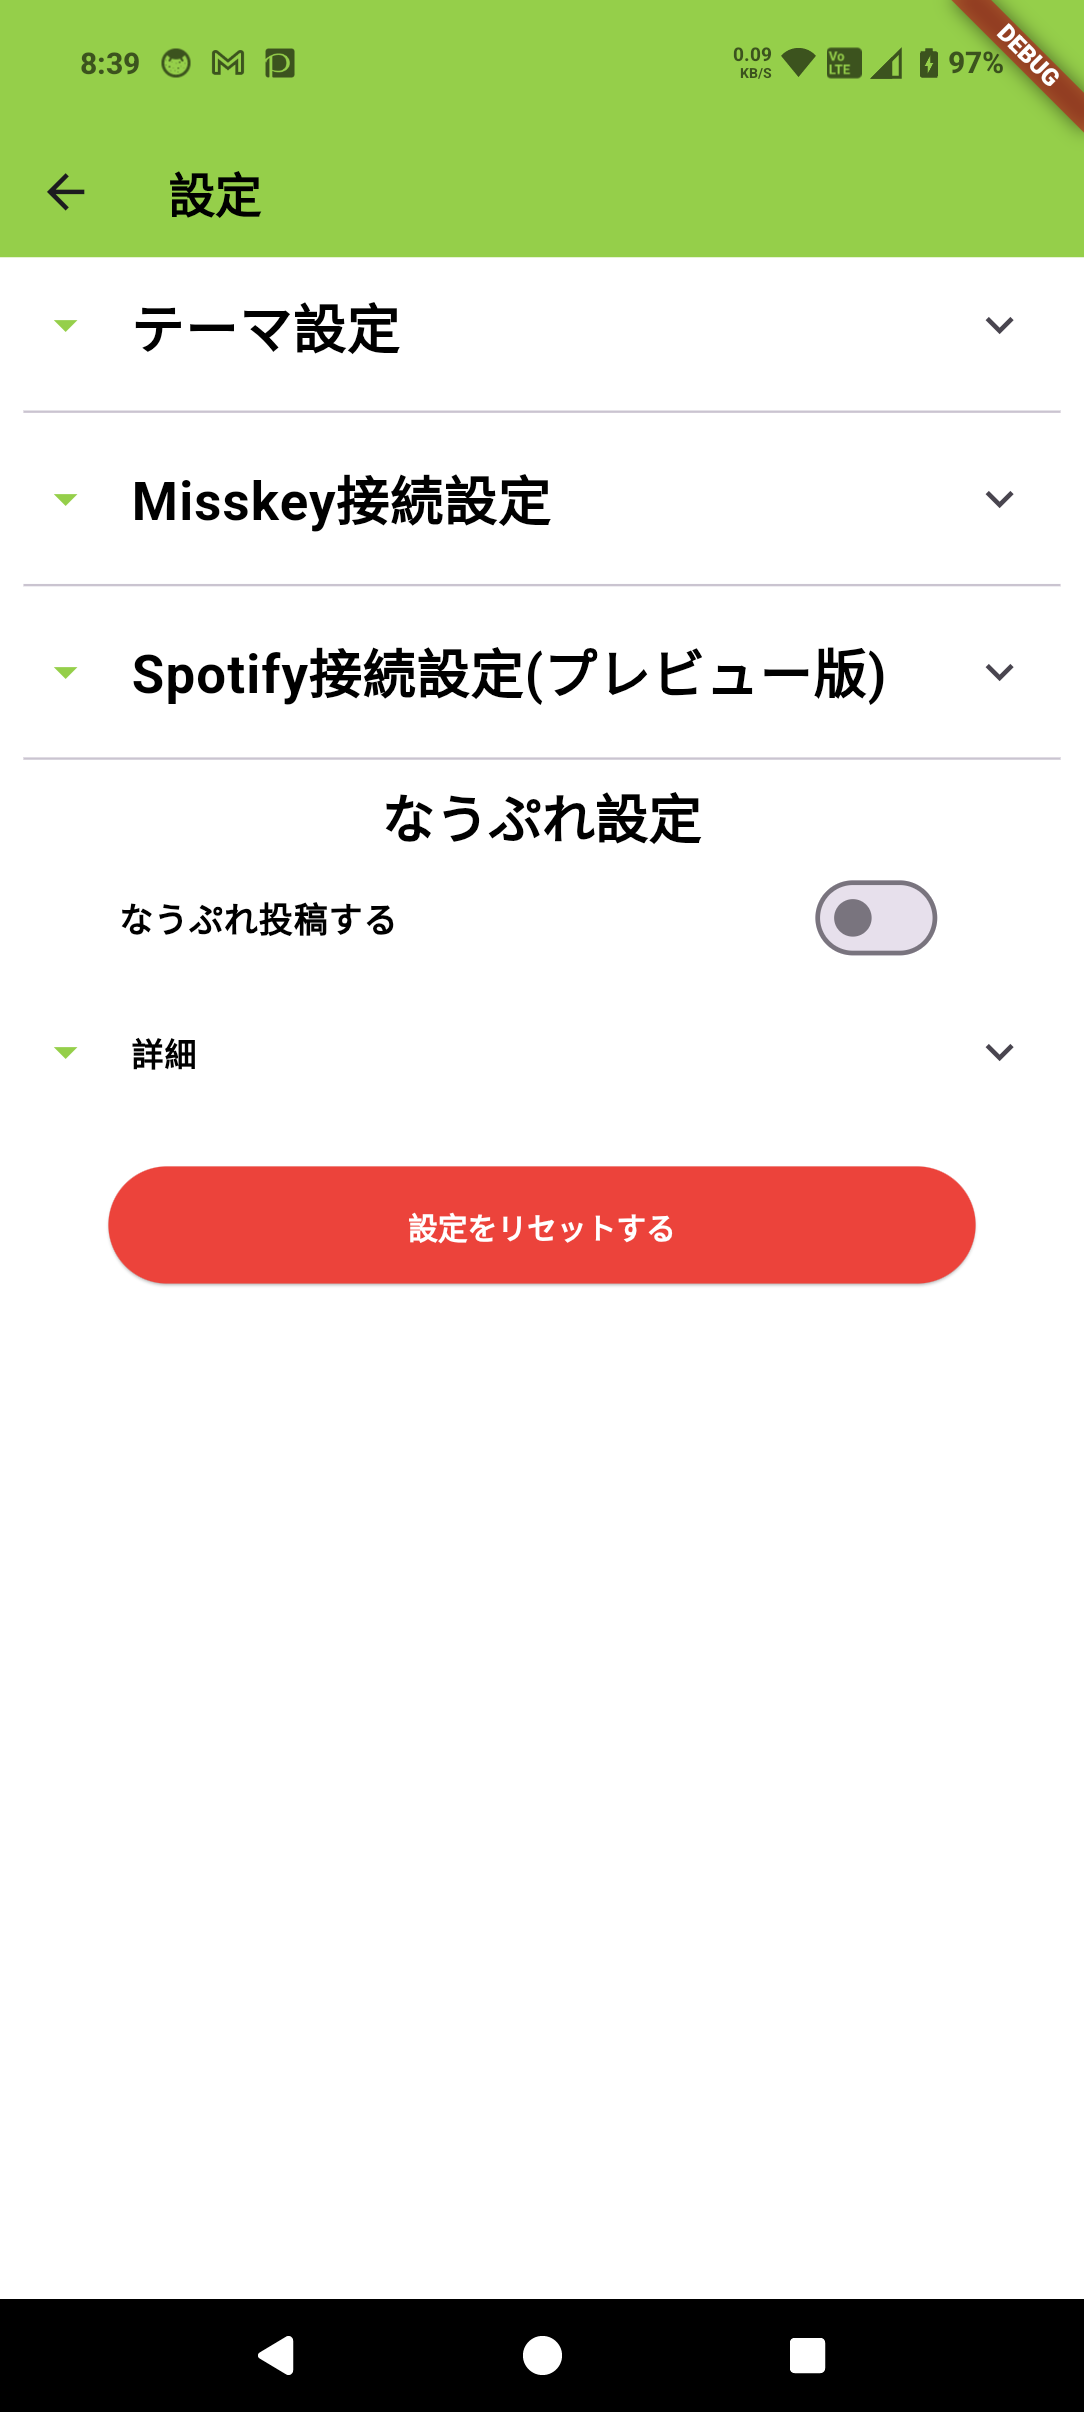
\includegraphics[width=5cm]{./pictures/misskey1.png}
                            }
                            \caption{展開前}
                            \label{img:misskey1}
                        \end{minipage}
                        \begin{minipage}[b]{0.45\linewidth}
                            \centering
                            \fbox{
                                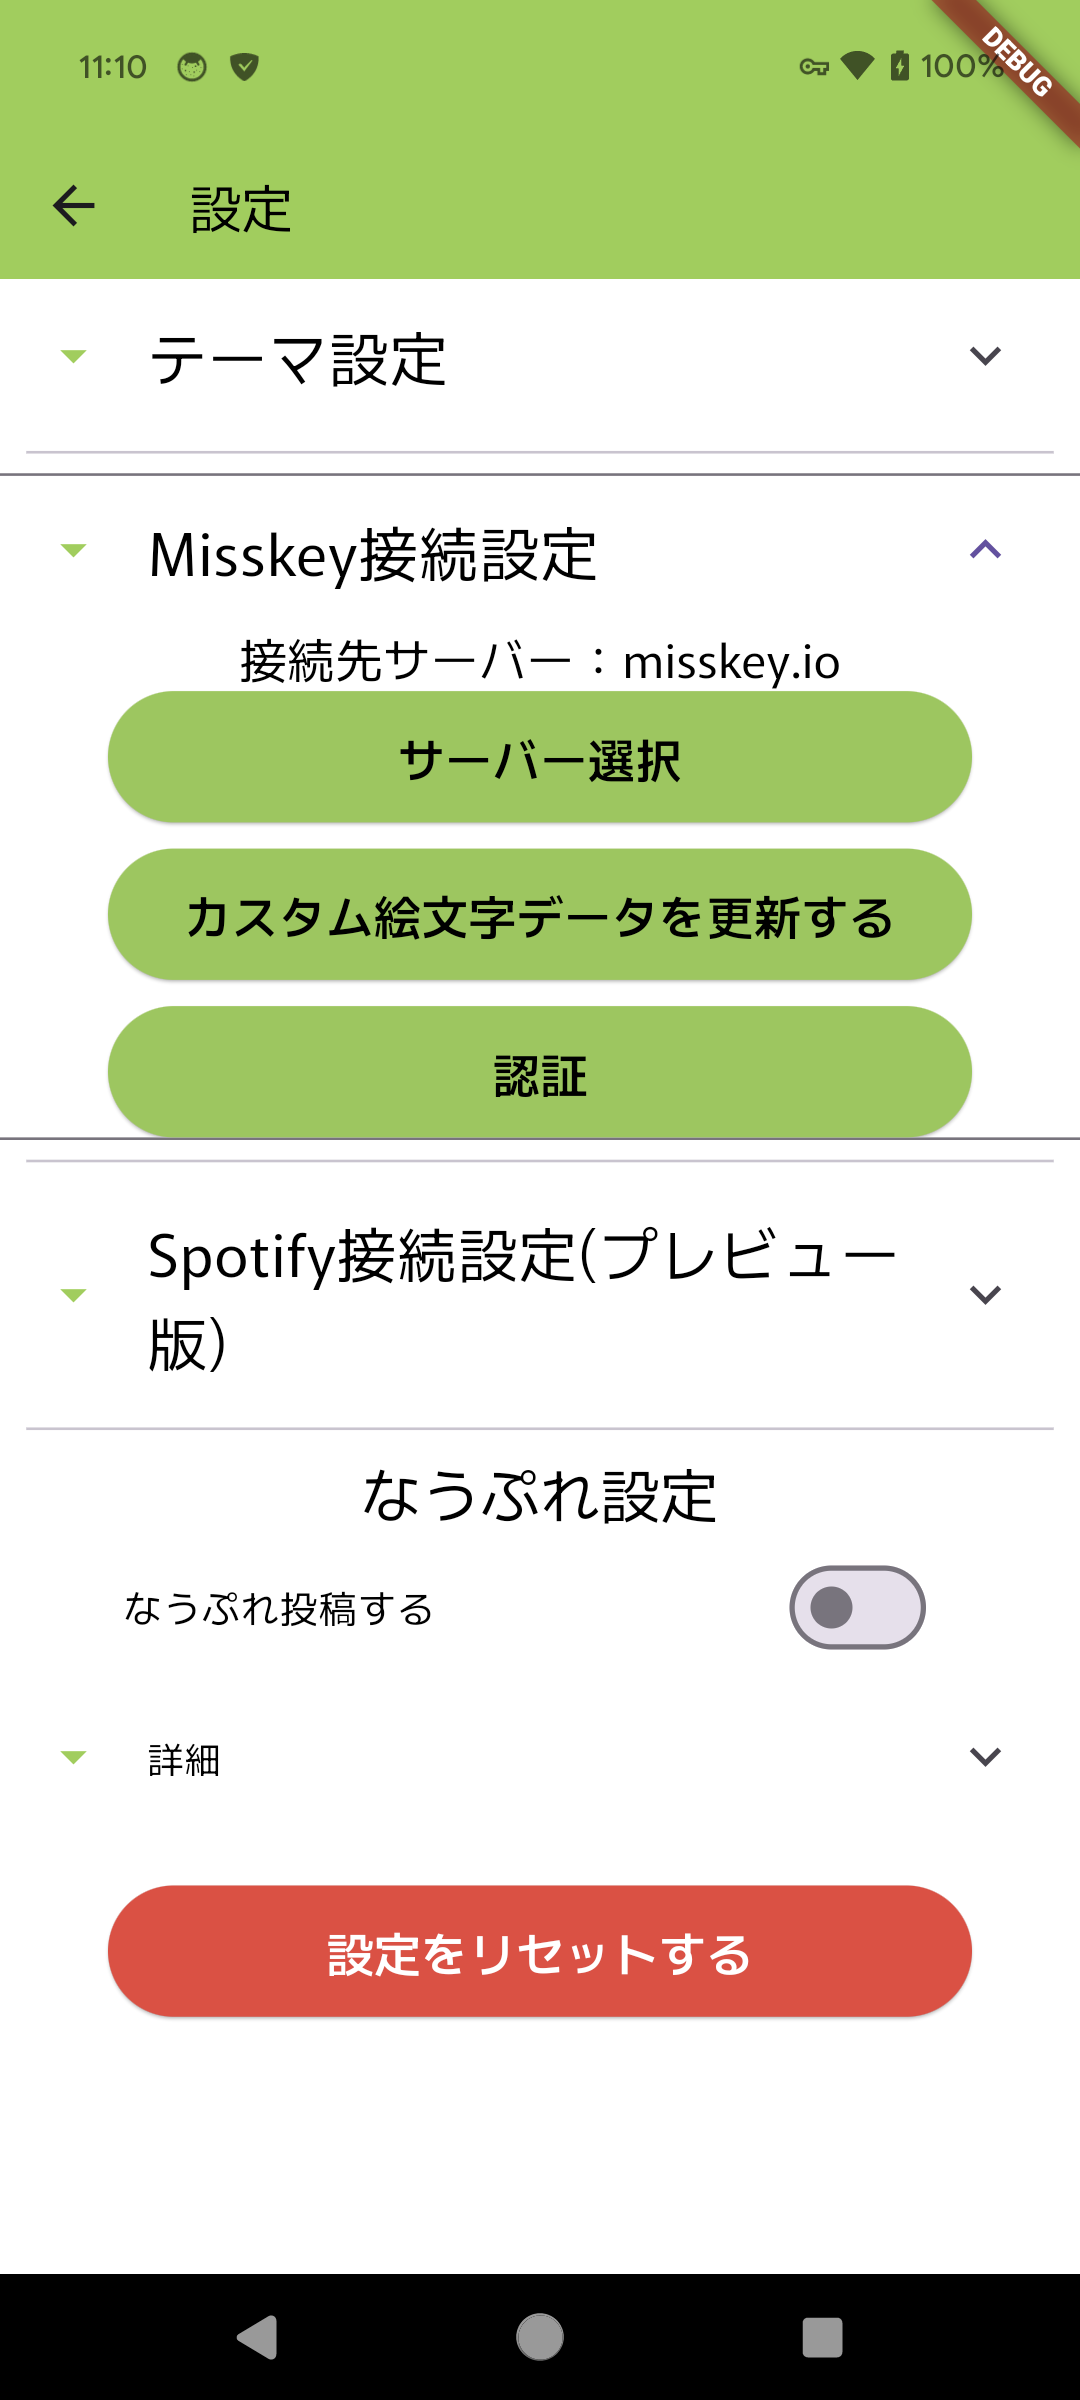
\includegraphics[width=5cm]{./pictures/misskey2.png}
                            }
                            \caption{展開後}
                            \label{img:misskey2}
                        \end{minipage}
                        \caption*{\mi 接続設定(\currentVersion)}
                    \end{figure}

                \item \ttbox{認証する}ボタンを押下してアプリへのアクセス許可ページにアクセスしてください。
                \label{item:misskey3}

                \newpage
                \item \nowplaying したい\mi アカウントのユーザー名、パスワードを入力して\ttbox{ログイン}を押下してください。
                \label{item:misskey4}
                    \begin{figure}[htbp]
                        \centering
                        \fbox{
                            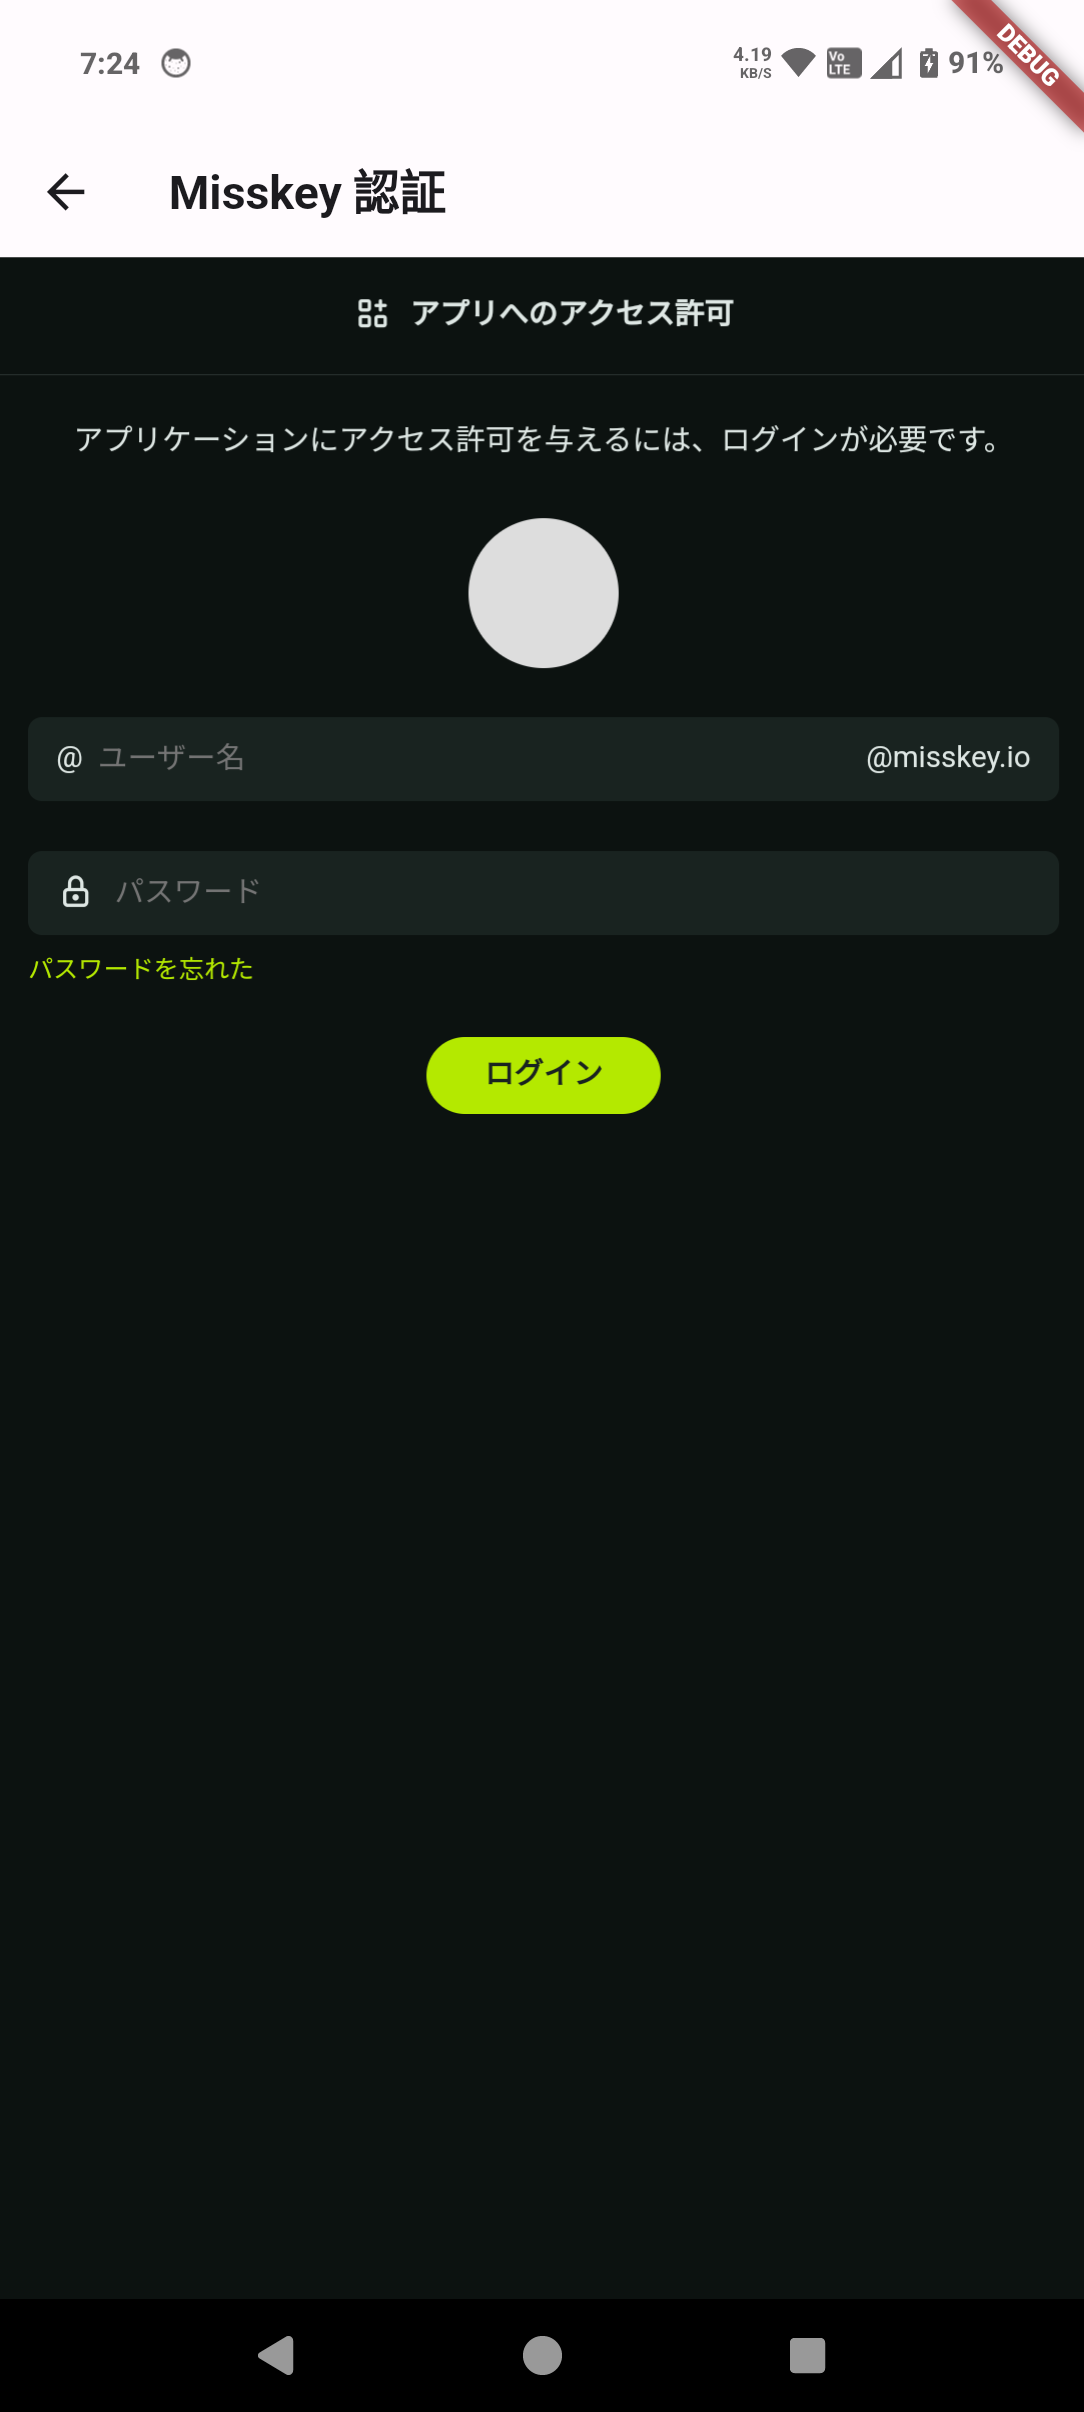
\includegraphics[width=5cm]{./pictures/misskey3.png}
                        }
                        \caption{ログインページ}
                        \label{img:misskey3}
                    \end{figure}

                \newpage
                \item \imageref{img:misskey4}のように二要素認証の入力を要求された場合は、\bracketref{item:misskey1}で作成した認証コードを入力して\ttbox{ログイン}を押下してください。
                    \begin{figure}[htbp]
                        \centering
                        \fbox{
                            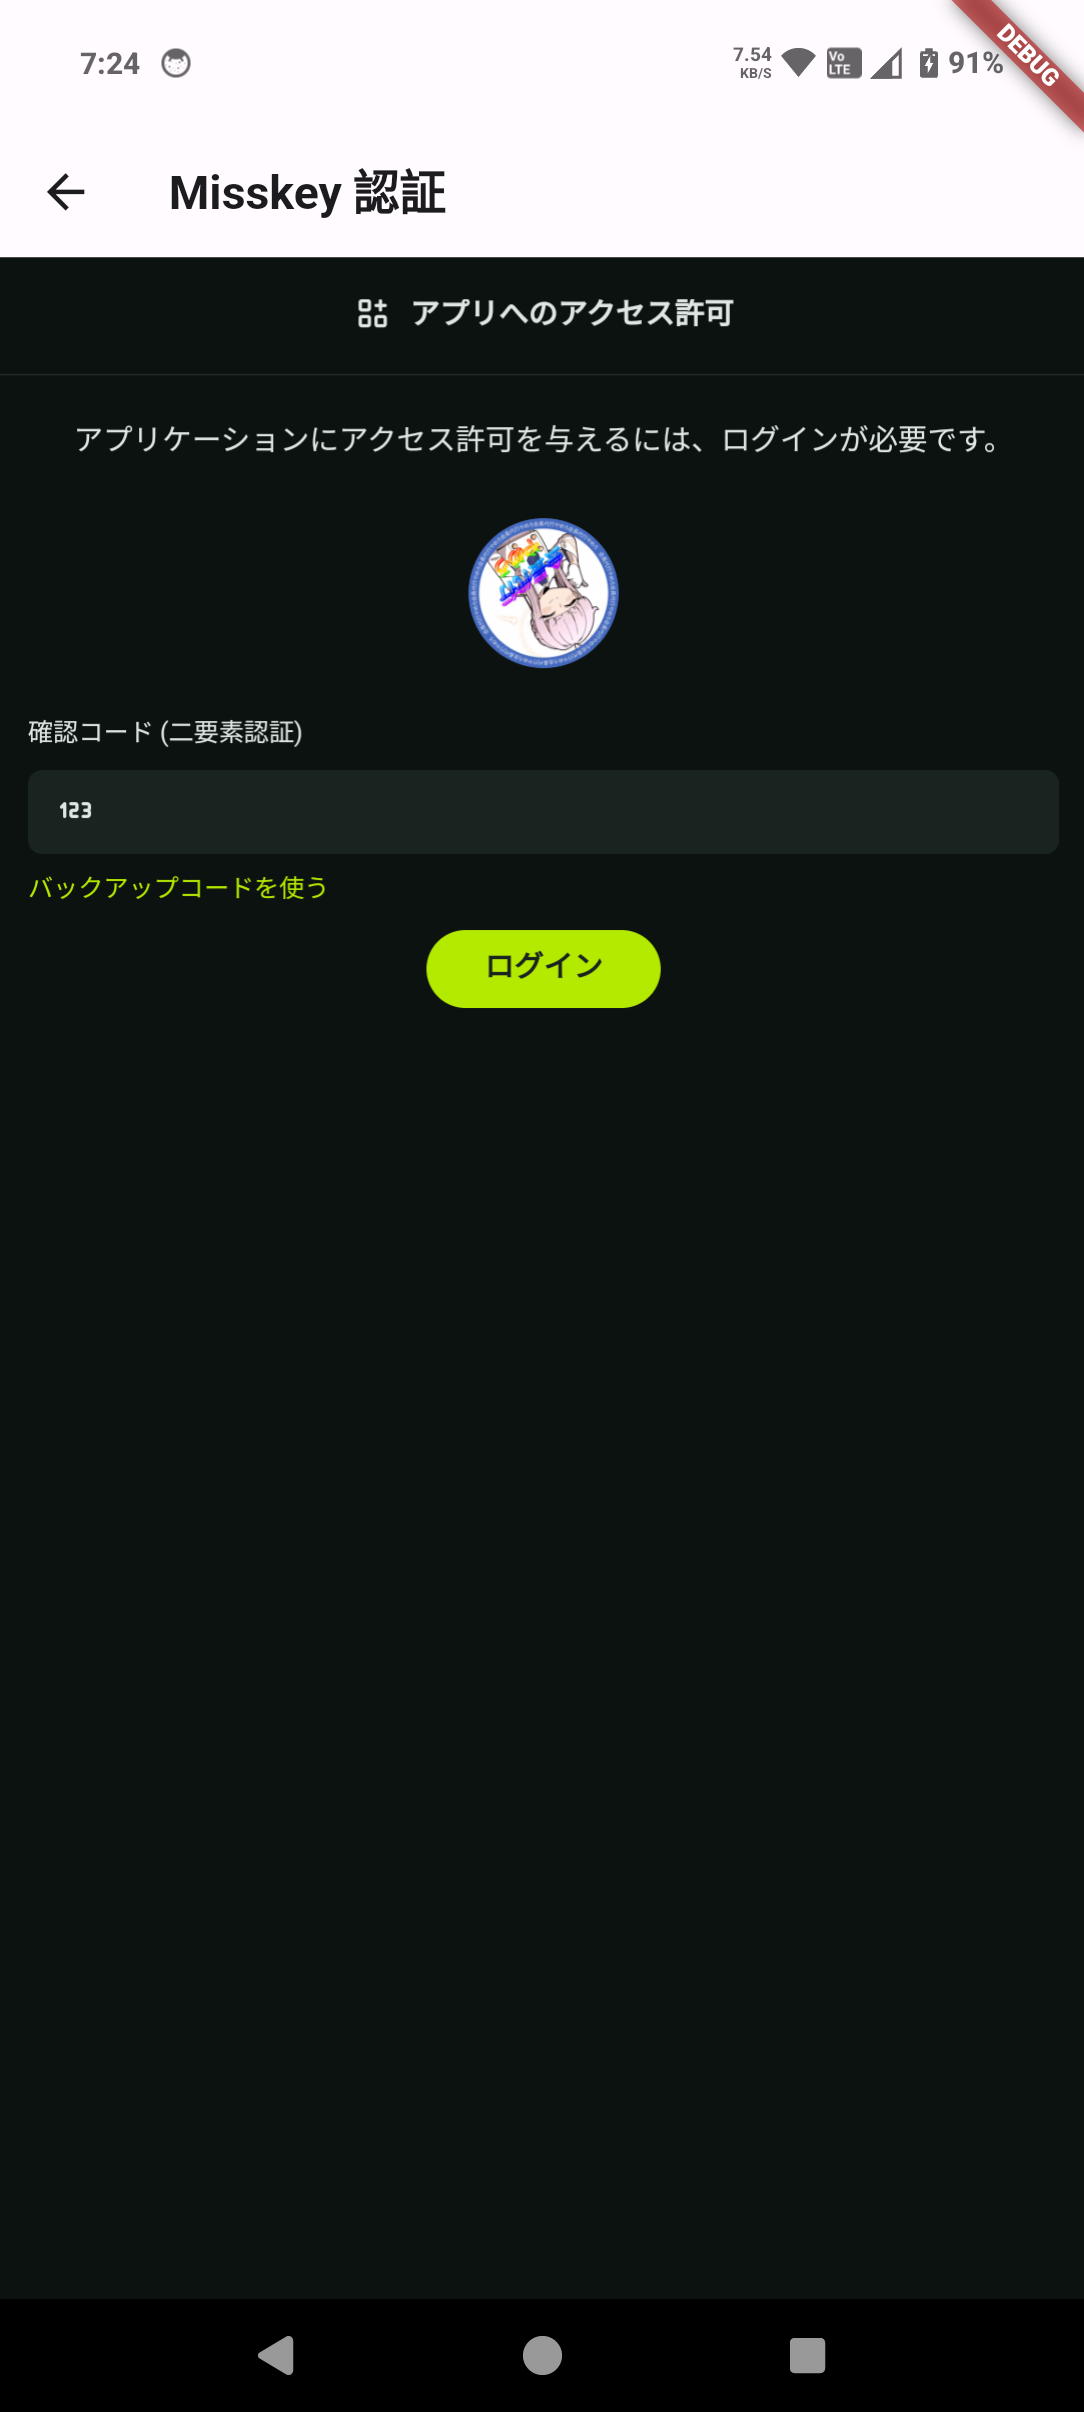
\includegraphics[width=5cm]{./pictures/misskey4.png}
                        }
                        \caption{二要素認証入力ページ}
                        \label{img:misskey4}
                    \end{figure}

                \newpage
                \item \imageref{img:misskey5}のようなアクセス許可ページが表示されるので、\ttbox{許可}を押下してください。
                    \begin{figure}[htbp]
                        \centering
                        \fbox{
                            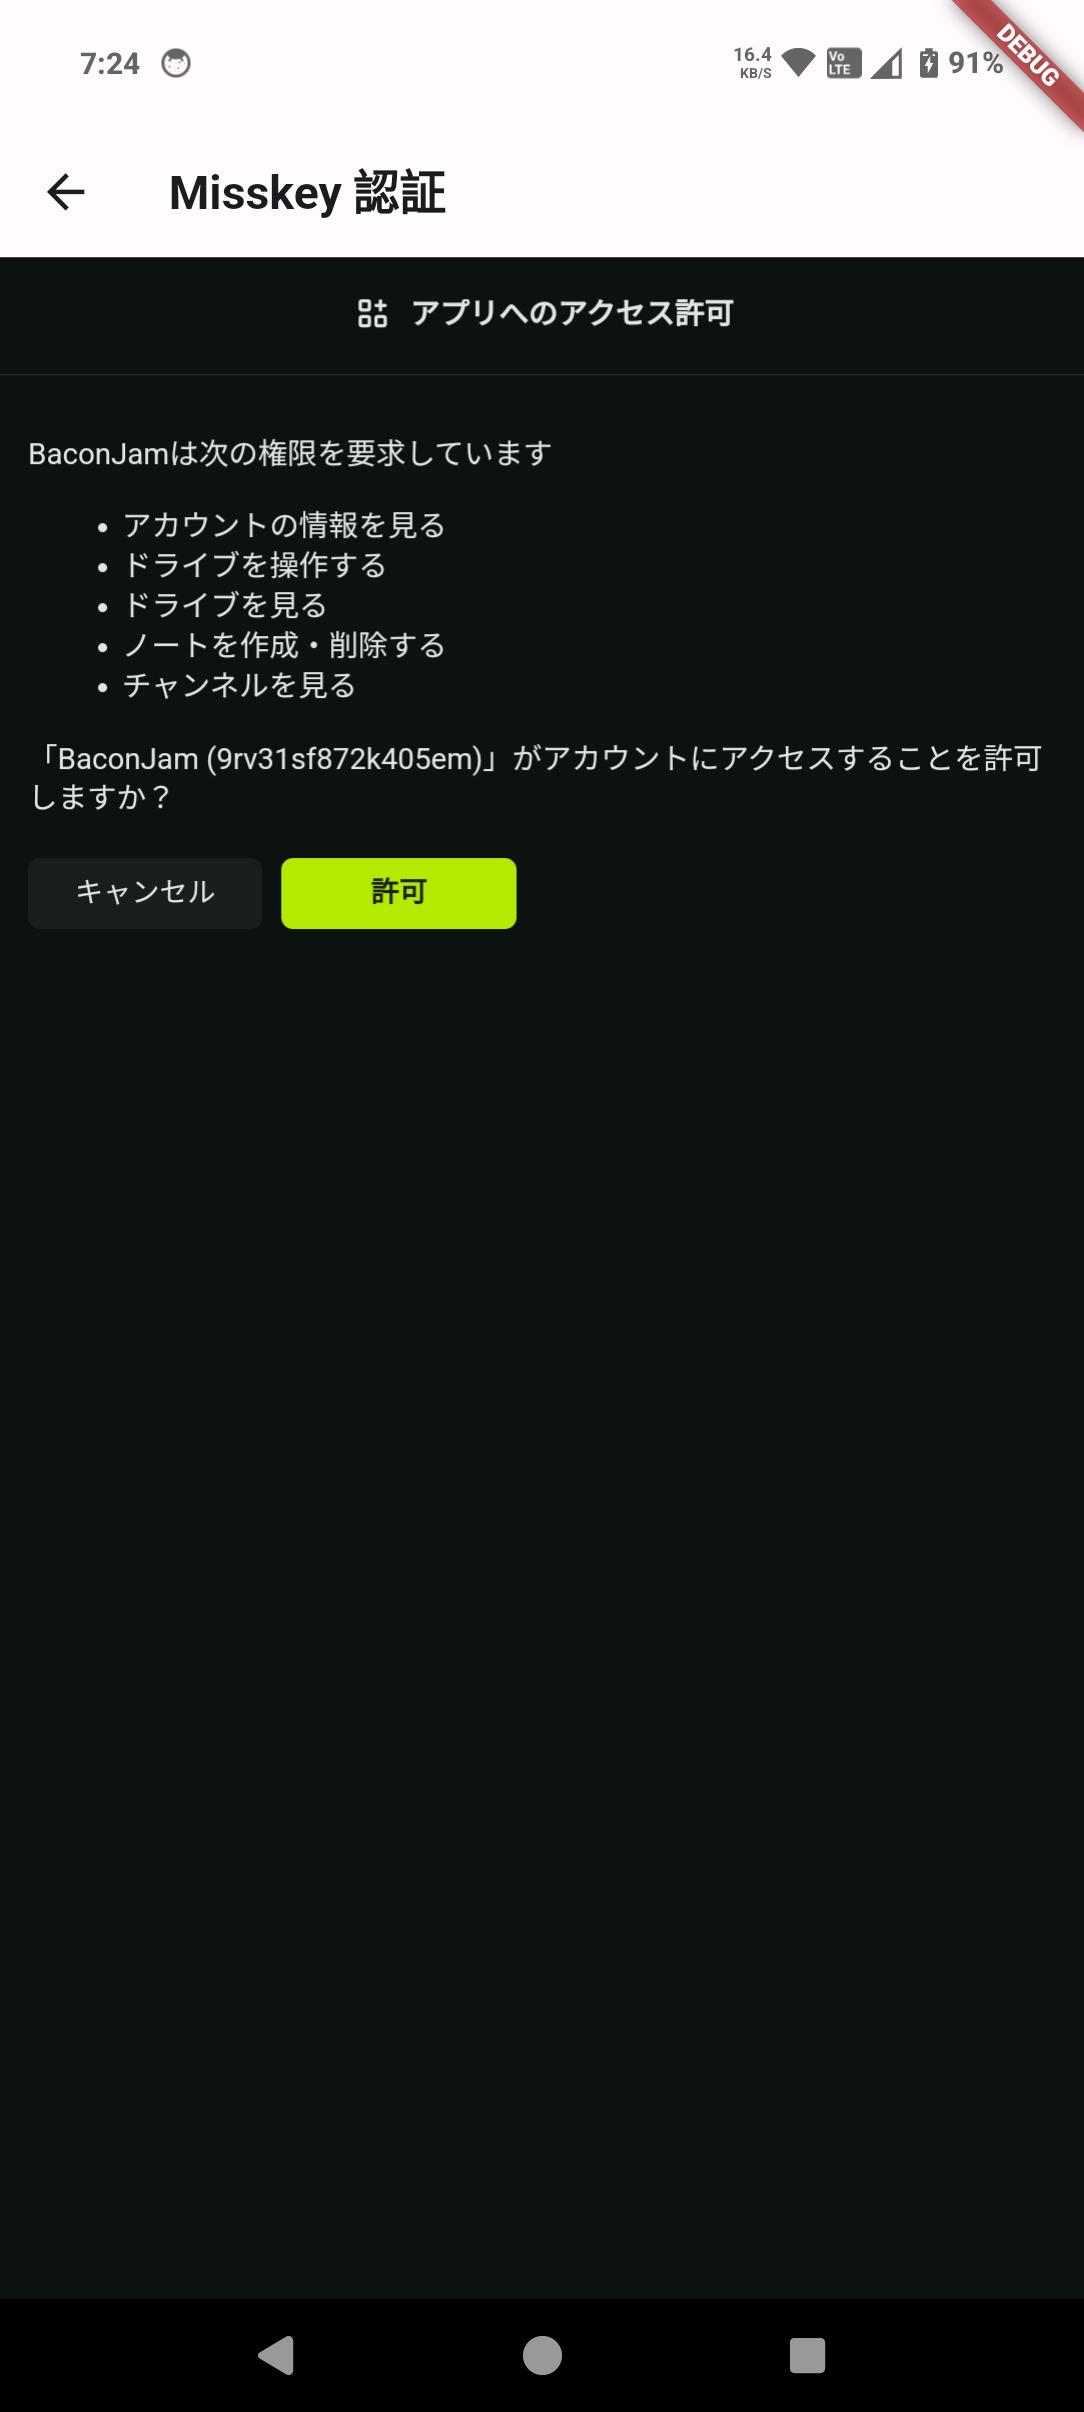
\includegraphics[width=5cm]{./pictures/misskey5.png}
                        }
                        \caption{アクセス許可ページ}
                        \label{img:misskey5}
                    \end{figure}

                \newpage
                \item \imageref{img:misskey6}のような認証完了ページが表示されたら、\bj に戻ってください。
                    \begin{figure}[htbp]
                        \centering
                        \fbox{
                            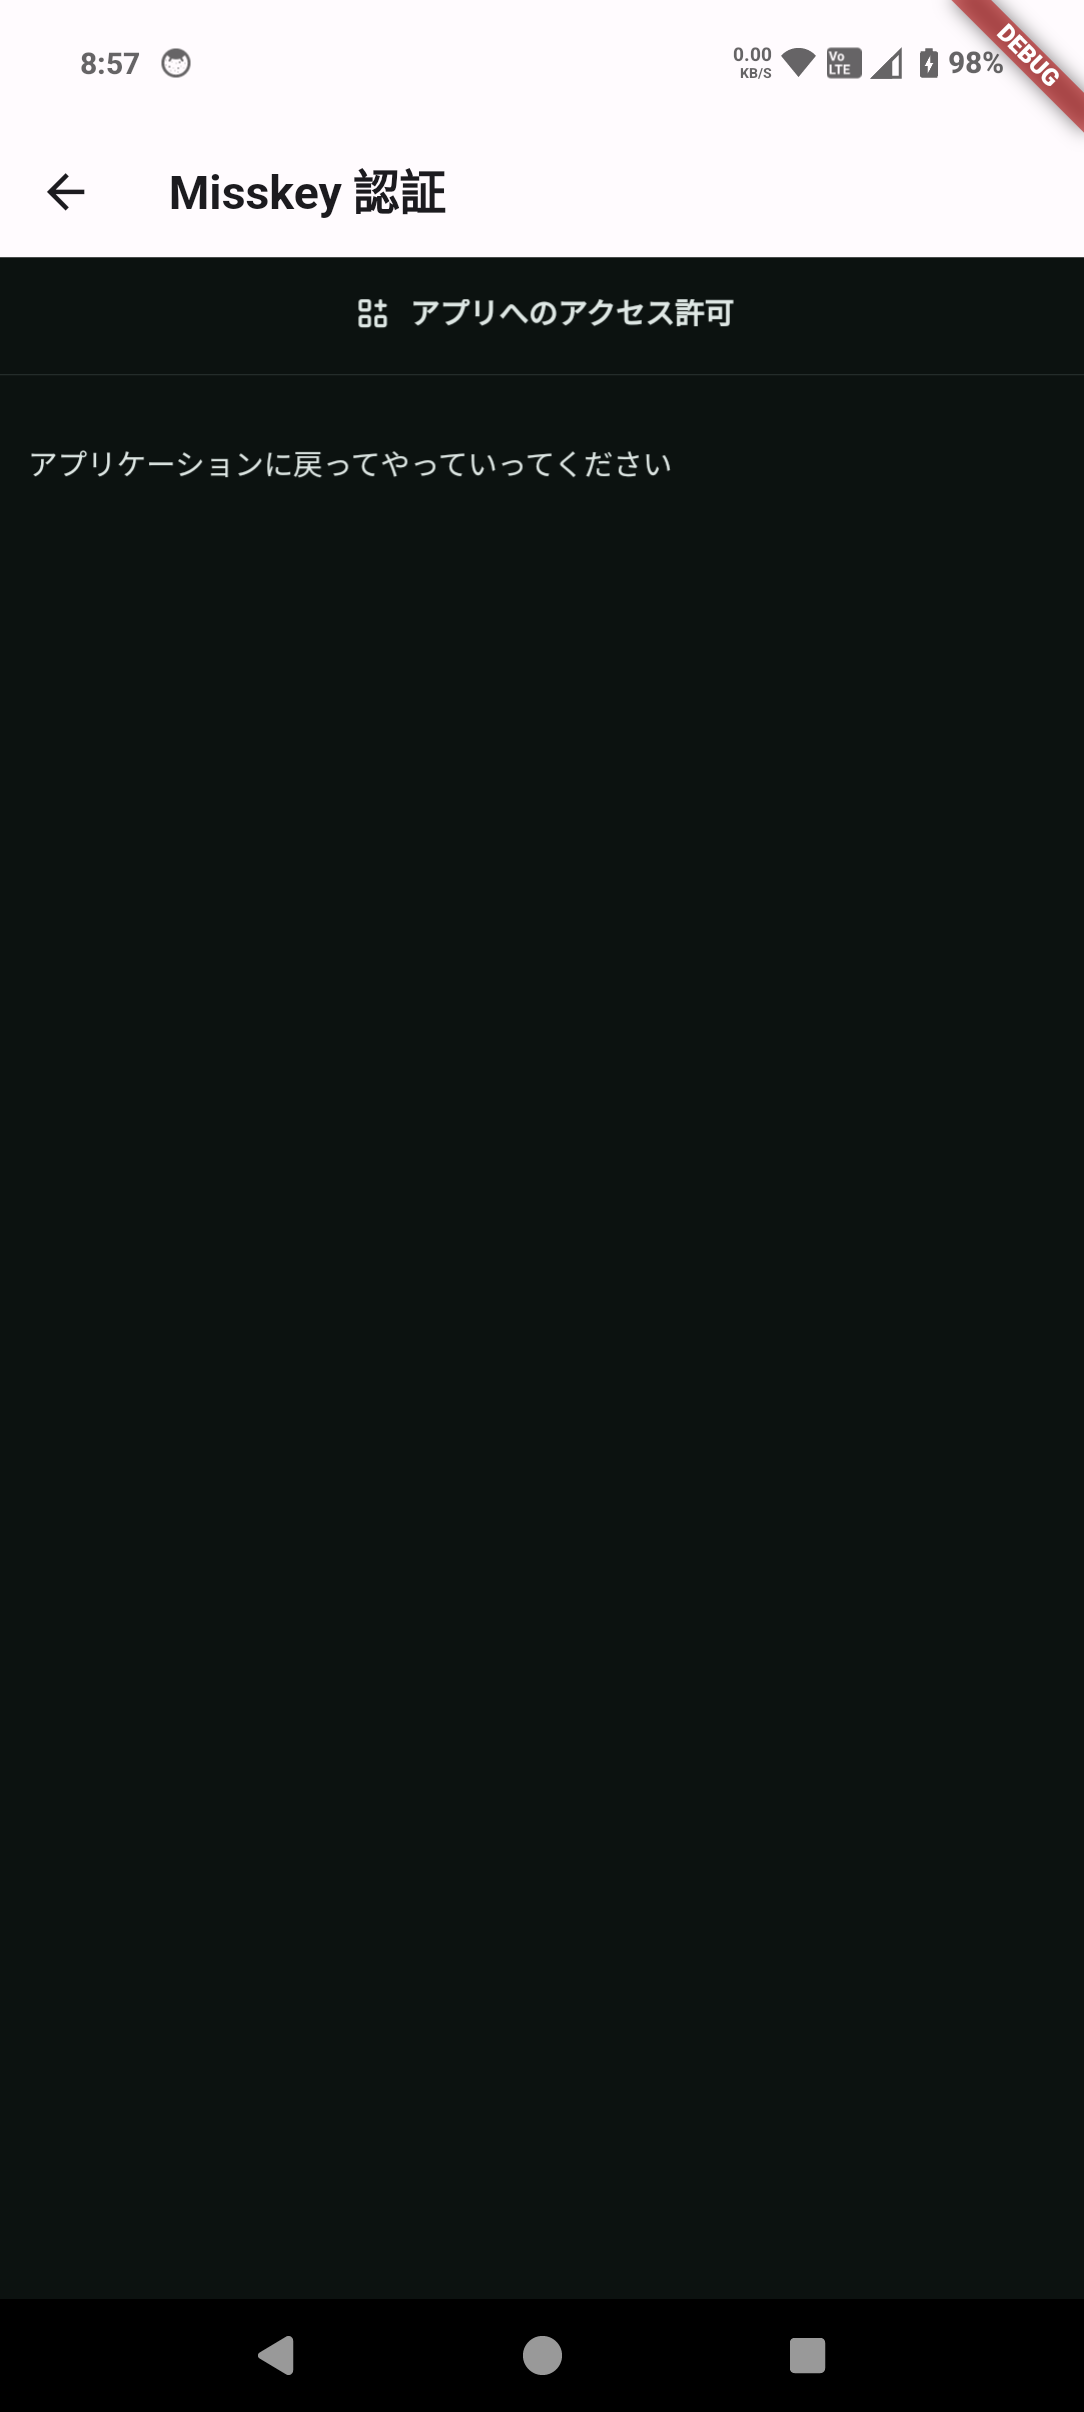
\includegraphics[width=5cm]{./pictures/misskey6.png}
                        }
                        \caption{アクセス許可ページ}
                        \label{img:misskey6}
                    \end{figure}

                \newpage
                \item \ttbox{Misskey接続設定}の\ttbox{してきたよ}を押下すると\imageref{img:misskey7}のようなダイアログが表示され、ご自身のアカウントが正しく連携されていることを確認してください\footnote{確認を完了しないと投稿が実行されません}。
                    \begin{figure}[htbp]
                        \centering
                        \fbox{
                            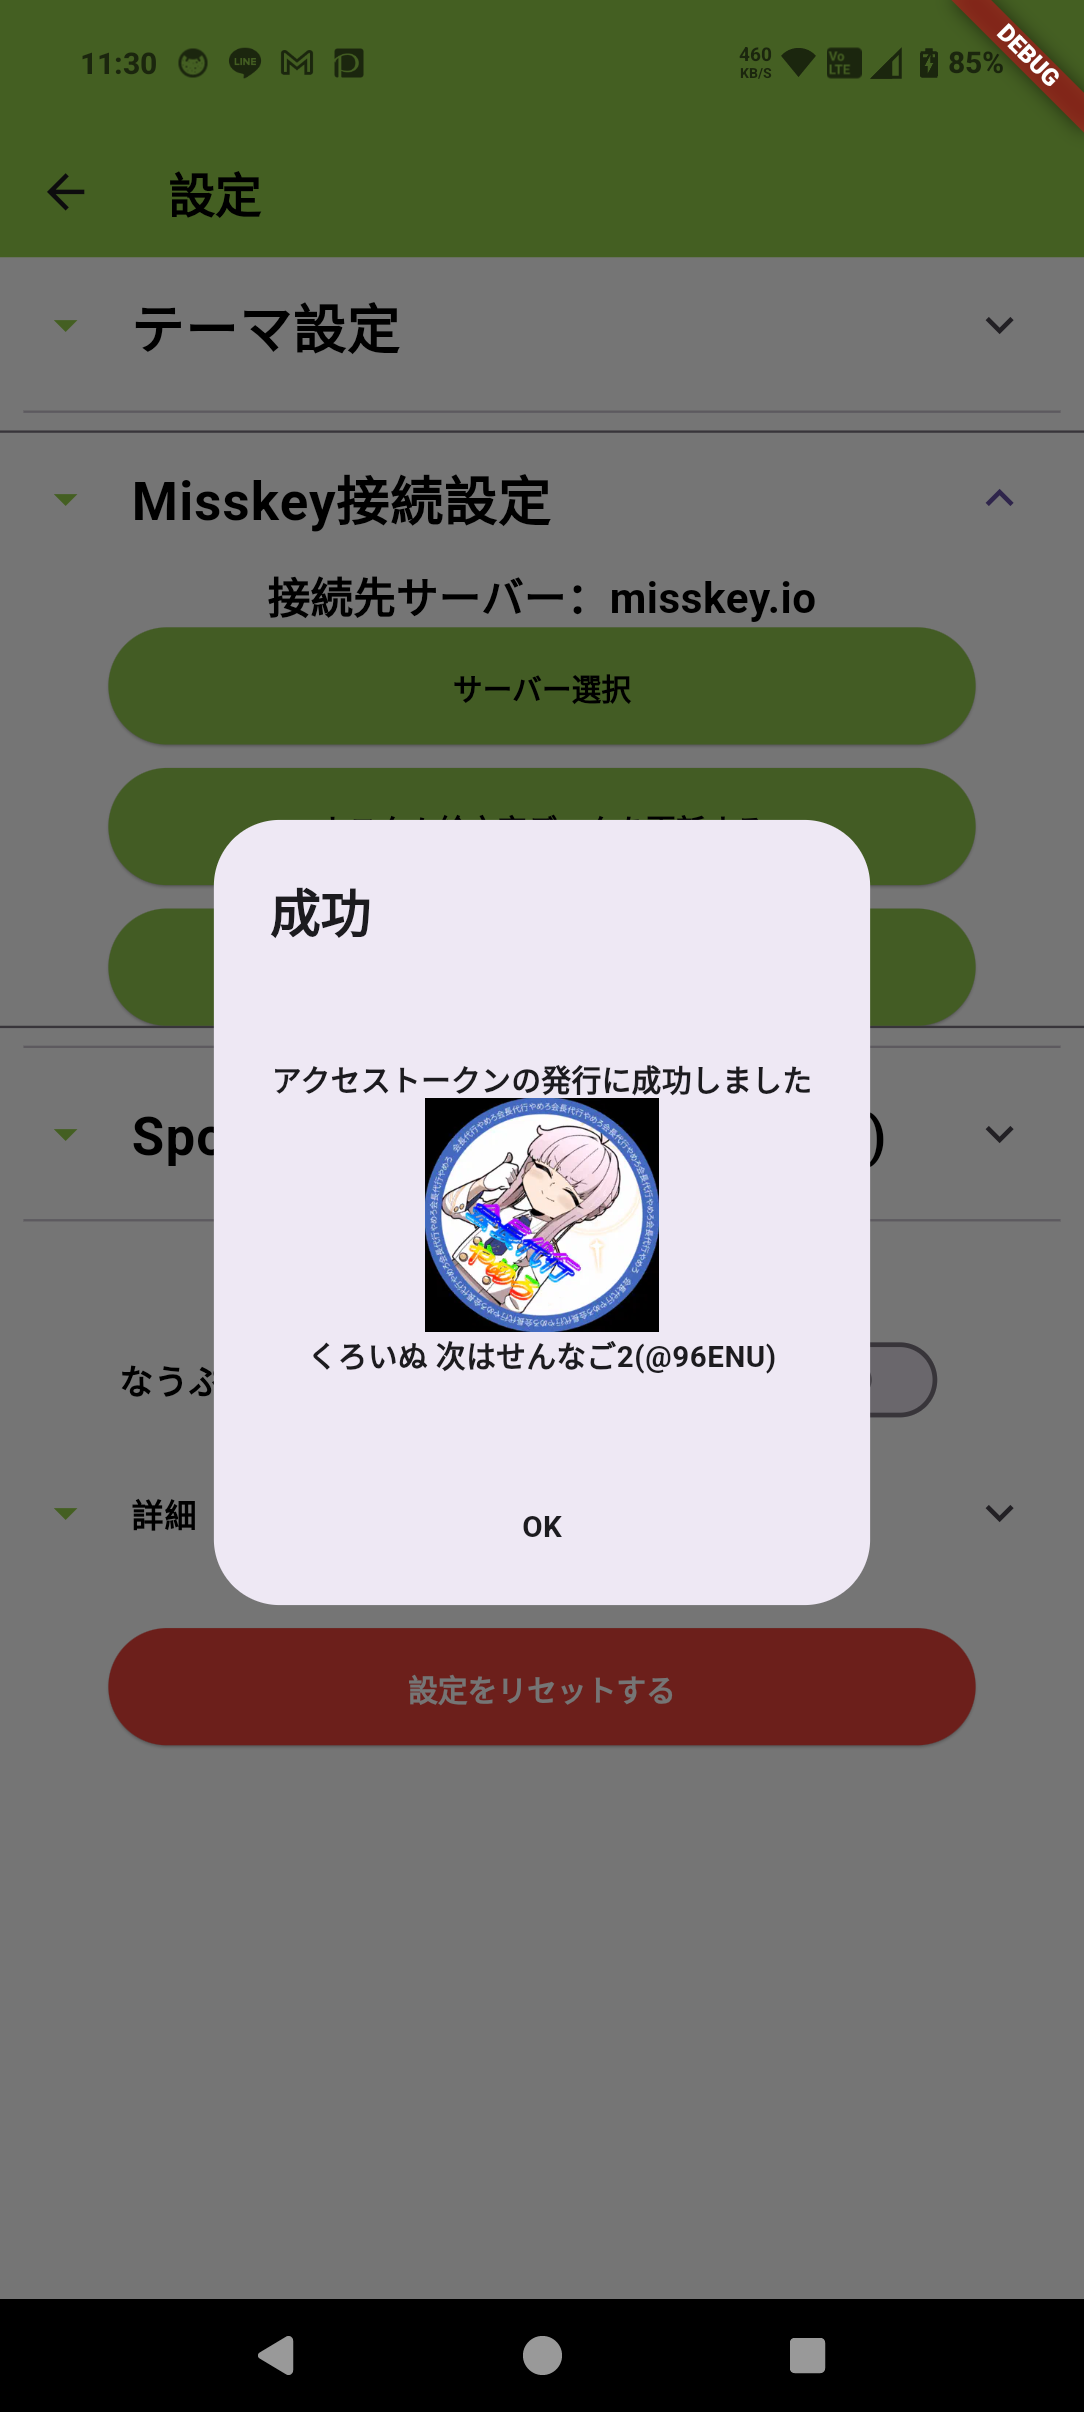
\includegraphics[width=5cm]{./pictures/misskey7.png}
                        }
                        \caption{アプリ連携完了ダイアログ}
                        \label{img:misskey7}
                    \end{figure}
            \end{enumerate}

        \newpage
        \subsubsection{発行した\accessToken の確認・削除}
        \label{sec:misskey4}
            \begin{enumerate}
                \item 連携先の\mi サーバーで\ttbox{設定}→\ttbox{API}を押下してください。
                    \begin{figure}[htbp]
                        \centering
                        \fbox{
                            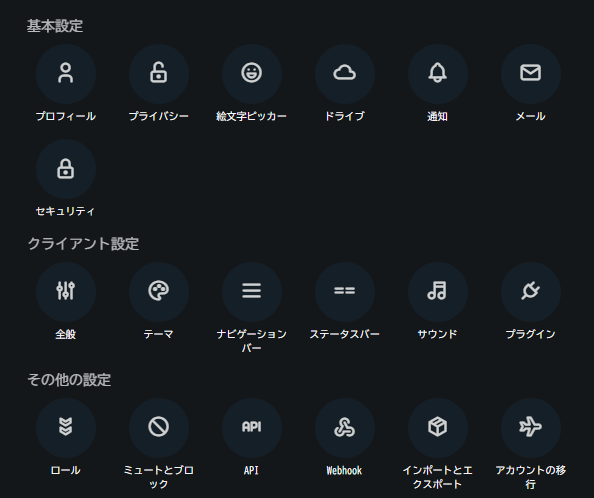
\includegraphics[width=5cm]{./pictures/misskey8.png}
                        }
                        \caption{設定ウィンドウ}
                        \label{img:misskey8}
                    \end{figure}

                \item \ttbox{\accessToken の管理}を押下してください。
                    \begin{figure}[htbp]
                        \centering
                        \fbox{
                            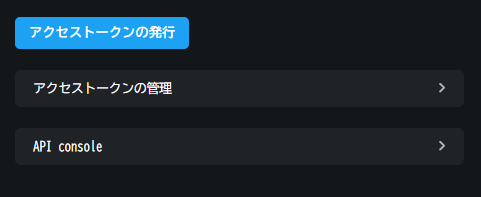
\includegraphics[width=5cm]{./pictures/misskey9.png}
                        }
                        \caption{APIウィンドウ}
                        \label{img:misskey9}
                    \end{figure}

                \item \accessToken 覧に、\bj という名前のものが発行されています。不要になった場合は、ゴミ箱アイコンを押下して\accessToken を削除してください。
                    \begin{figure}[htbp]
                        \centering
                        \fbox{
                            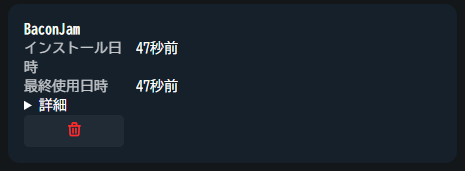
\includegraphics[width=5cm]{./pictures/misskey10.png}
                        }
                        \caption{アクセストークン}
                        \label{img:misskey10}
                    \end{figure}
            \end{enumerate}